One of the objectives of this thesis is the implementation and analysis of a prototype App for mobile devices. In this chapter, the previously selected algorithms will be put into the context of the App's implementation, and the App's structure itself will be detailed. This chapter is structured as follows:

\begin{itemize}
	\item \textbf {About Android Apps} - An introduction to the Android operating system.
	\item \textbf {Assembly of Algorithms and Information Flow In Concrete Implementation} - Gives details on algorithms and information flow between them, as previously listed in an overview in Chapter ~\ref{ch:scenario}.
	\item \textbf {Illustrations of Algorithm Steps} - Lists illustrations and descriptions of the algorithm succession in the App prototype.
	\item \textbf {Retrieval of Music Metadata} - Describes how music metadata is retrieved from a mobile device's storage and from web sources.
	\item \textbf {Retrieval of Similarity Data} - Describes how artist similarity data is retrieved from web sources, and how unknown values are approximated.
	\item \textbf {Implementation of Multidimensional Scaling} - Contains a pseudo-code listing of one step in the MDS algorithm.
	\item \textbf {Implementation of Removal of Node Overlappings} - Contains a pseudo-code listing of the algorithm implementation which removes overlappings of graph nodes.
	\item \textbf {Visualization Details} - Features implementation details of the prototype concerning visualization of graph data.
	\item \textbf {Structure of the App} - Presents the structure of the prototypical App, together with information about the target operating system.
\end{itemize}

\section{Assembly of Algorithms and Information Flow In Concrete Implementation}
\label{sec:algorithm-assembly}

In Chapter ~\ref{ch:scenario}, an overview was given of how algorithms work together in the system. In-depth implementation-specific details of this assembly and information flow will now be given. These steps are in part also illustrated in Fig. ~\ref{fig:screen_mds_1_initial} to Fig. ~\ref{fig:screen_mds_10_after_all_uncollided_nodes}.

\subsection{About Android Apps}

Android is a mobile operating system developed by the Open Handset Alliance ~\cite{url:openhandsetalliance}, led by Google. Its architecture allows for 3rd party programs (called "'apps"') to easily be run and debugged on Android devices.
Android apps are run in the Dalvik VM \footnote{A Virtual Machine (VM) is the emulation of computing hardware on which software can be run which is tailored to the emulated architecture, without ever owning the actual hardware. Virtual Machines are usually executed as programs on a host operating system. Android's Dalvik VM allows to execute computer code without the need to compile it up front, like the Java VM, from which it is derived.} which makes use of a register-based architecture, relying on a Linux kernel for low-level functionality ~\cite{dalvik}. The most wide-spread programming language for building Android apps is Java, but various other languages such as Scala or even scripting languages like Groovy or Lua can be used. Since mid 2009, developers can also write and integrate native C and C++ code by making use of the Native Development Kit (NDK).

From an app developer's perspective, the frameworks contained in Android dictate a user-centric application structure, made up of so-called Activities ~\cite{url:androidactivity}. Every Activity encapsulates a screen which is presented to the user. Activities are loosely coupled, allowing only serialized objects and primitive values to be passed between them.

User interface composition in Android is performed partly in the CPU (e.g., in Java code), and partly in the device's GPU (by using the OpenGL interface). Apps can also choose between these composition variants.

Android is a strictly touch-centric operating system, meaning that most user interactions are performed via the device's touch screen. Originally, Android devices were bound to provide hardware buttons, but starting with Android 4.0, those buttons are gradually replaced with software buttons (displayed on the touch screen).

This prototype is built and tested with Android 4.0.

\subsection{Library Visualization}
\label{subsec:libraryvis}

\begin{itemize}
	\item Extraction of music metadata on the device \\\\
			\textbf{Input:} Access to a data store containing the device's music library metadata. \footnote{The app prototype utilizes a standard SQLite database in order to store data which can be persisted in order to reduce computation time, thus improving the user experience.}
			  \\
			\textbf{Algorithm:} Iterates through all artists and tracks in the device's music library.
			If an entity has not yet been registered in the app's database, parts of its metadata (for all entities: name, Last.fm entity ID, Echonest entity ID, Last.fm imageURL; for artists: albums, tracks; for albums: artist, tracks; for tracks: artist, album) are compiled and put into the database. \\
			\textbf{Output:} Local music metadata stored in the app's database.\\
			
	\item Matching of the device's music metadata with metadata from web sources \\\\
			\textbf{Input:} Local music metadata stored in the app's database.  \\
			\textbf{Algorithm:} Iterates through all local music metadata previously retrieved (artists, albums, titles...), and calls	Last.fm's and Echonest's RESTful API to find matching entities - picking the first match as best match (obviously, this first match could be wrong - in empirical tests, this problem did not occur, but a more resilient matching algorithm should be explored in further research). The name and Last.fm/Echonest ID of this first match is then stored in the app's database, with a relational link to the respective music entity residing in the device storage. \\
			\textbf{Output:} Remote music metadata stored in the app's database. \\
			
	\item Querying of Artist Similarity data from web sources \\\\
			\textbf{Input:} Local music metadata and matched metadata from remote web sources stored in the app's database. \\
			\textbf{Algorithm:} Iterates through all local and remote music metadata previously retrieved, and calls
			Last.fm's RESTful API to get a similarity ranking list of the 100 most similar artists (with each item consisting of a similarity measure, the artist's name, and other artist metadata which is not used in this algorithm) for each locally available artist in the local database. From this retrived list, only the similarity measure and name of each respective artist is evaluated: If an item in this list has a name attribute that equals to a locally available artist's name (case-insensitive String equality), then this item is treated as a representation of exactly this artist. Subsequently, a similarity relation from the locally availabe artist (for whom the similarity ranking query was issued) to the artist identified in the respective list item is created, with a similarity measure that is copied from that same list item. The similarity measure has a range of [0..1], where 1 means "'most similar or equivalent"' and 0 means "'not related at all"'.\\
			\textbf{Output:} Artist similarity relations stored in the app's database. \\
			
	\item Completion of Artist Similarity data \\\\
			\textbf{Input:} Artist similarity relations stored in the app's database. \\
			\textbf{Algorithm:} Iterates through the previously retrieved artist similarity relations, and
			adds approximations for similarity relations which have not been found in the web API's results.
			These approximations are calculated as described in section ~\ref{sec:matching-music-entities}. \\
			\textbf{Output:} Complete artist similarity relations stored in the app's database. \\
			
	\item Laying out artists in 2D space with a Multi Dimensional Scaling (MDS) algorithm \\\\
			\textbf{Input:} Complete artist similarity relations stored in the app's database.   \\
			\textbf{Algorithm:} Applies a multistep (see sub-steps) algorithm which uses previously
			retrieved similarity data to position nodes resembling artists without overlappings.  \\
			\textbf{Output:} Graph structure of nodes resembling artists, laid out such that their position 
			indicates their similarity to each other. \\
			
			This step will be performed by the following sub-steps.

		\begin{itemize}
			
			\item Building up of a distance matrix (in-memory structure) between artists such that subsequent algorithm steps need not query the device's storage for similarity measures. \\\\
				\textbf{Input:} Complete artist similarity relations stored in the app's database. \\
				\textbf{Algorithm:} Iterates through all artist similarity relations, calculates a
				distance value (\emph{d = 1 - Similarity}, d $\in$ [0, 1], Similarity $\in$ [0, 1]), and writes it into
				a matrix data structure where both dimensions' labels consist of all existing artists. \\
				\textbf{Output:} Distance matrix of artists, based on their inverted similarities. \\
				
			\item Generation of a subset of artists and laying them out according to spring model forces	\\\\
				\textbf{Input:} Distance matrix of artists, based on their inverted similarities. \\
				\textbf{Algorithm:} Picks a random sample of artists of size $\sqrt{N}$ (N: number of all artists), assigns random positions to them,
				and applies a multi-dimensional scaling algorithm on them (see subsection 
				~\ref{subch:implementation-mds} later in this section). \\
				\textbf{Output:} Graph structure of nodes resembling artists (correctly positioned subset) \\
				
			\item Addition of the remaining artists, positioning them around the initial subset \\\\
				\textbf{Input:} Graph structure of nodes resembling artists (correctly positioned subset) \\
				\textbf{Algorithm:} Iterates through the remaining artist nodes and positions each on a position
				in the vicinity of its most similar artist (estimating which quadrant will be the best, as described in Chapter ~\ref{ch:computation}). \\
				\textbf{Output:} Graph structure of nodes resembling artists, many of them suboptimally positioned \\
				
			\item Application of spring model forces on all nodes for a few iterations \\\\
				\textbf{Input:} Graph structure of nodes resembling artists, many of them suboptimally positioned \\
				\textbf{Algorithm:} Applies the aforementioned multi-dimensional scaling algorithm on the whole graph of
				all artist nodes, thus reducing system stress \footnote{System stress is a metric for how well the current layout of a graph satisfies its internal forces. The higher the disconnect between the node's optimal distances and their actual distances is, the higher is the stress. One way to calculate stress is: S = $\sum_{n_i, n_j}^{n_N} ( Actual Distance(n_i, n_j) - Optimal Distance(n_i, n_j) ) ^ 2, n_i != n_j$} (finding a better position for each artist).  \\
				\textbf{Output:} Graph structure of nodes resembling artists, laid out such that their position 
				indicates their similarity to each other.\\
				
			\end{itemize}
				
	\item Removal of overlapping of artists' depictions in 2D space	\\\\
				\textbf{Input:} Graph structure of nodes resembling artists, laid out such that their position 
				indicates their similarity to each other. \\
				\textbf{Algorithm:} Empties out the graph, and re-adds the artist nodes back into it, one by one,	while optionally moving nodes when they are added such that they do not overlap any other nodes. This	movement is determined by the vector of both nodes' center coordinates and their amount	of overlapping. The concrete algorithm is shown in algorithm listing ~\ref{alg:removal-node-overlappings}. 

				\textbf{Note 1:} The concrete algorithm applies a random margin to repositioned nodes in order to prevent the forming of a equi-distant artist grid. In empirical observations, it has been found that users regard a equi-distant artist grid as too unnatural. An approach inspired by audio processing called "'humanization"' loosens up this rigid structure, that means that small random additions or subtractions are performed on the vector lengths moving the respective artists. The resulting object positions are not more than a few pixels different than without randomization, but the subjective result for the user improves.

				\textbf{Note 2:} After implementation, it turned out that this implemented removal of overlapping of nodes algorithm increases system stress severely, and in some cases also removes semantic meaning originally produced by the previous 2D layout generation algorithm. The only motivation for the removal of node overlappings are of cosmetical nature: visual overlappings could disturb the user's perception of the result, and hide nodes from the user when they are overlaid by other nodes. In future research, an algorithm better preserving the original layout (like the force transfer algorithm described in section ~\ref{sec:removal-node-overlapping}) should be evaluated and, if yielding better results, replace the algorithm described in this step.
				 \\
				\textbf{Output:} Graph structure of nodes resembling artists, laid out such that they don't 
				overlap each other and their position indicates their similarity to each other. \\
				
	\item Display of the laid out artists in OpenGL	\\\\
				\textbf{Input:} Graph structure of nodes resembling artists, laid out such that they don't 
				overlap each other and their position indicates their similarity to each other. \\
				\textbf{Algorithm:} Displays the graph on an OpenGL canvas (3D), by using the artists' images (in form
				of textures) and their names (rendered to textures). Sets the viewport and transformation
				matrices such that a 2D view is simulated, displaying artist nodes as viewed from above. \\
				\textbf{Output:} OpenGL view object and auxiliary system objects \\
				
	\item Continuous reaction to user actions (zooming, panning, tapping) \\\\
				\textbf{Input:} OpenGL view object and auxiliary system objects. \\
				\textbf{Algorithm:} Continuously reacts to user interface inputs, by moving the OpenGL canvas'
				pseudo-camera (i.e., manipulating the model transformation matrix) for zooming and panning.
				Marks an artist node as selected when the user taps onto it, and displays a context menu. \\
				\textbf{Output:} Updated view state
\end{itemize}

\subsection{Artist Discovery}

\begin{itemize}
	\item Queries last.fm for the N artists most similar to a "'seed artist"' which was previously selected by the user for this purpose.\\\\
				\textbf{Input:} The seed artist whom the user has selected for discovery. \\
				\textbf{Algorithm:} Queries Last.fm for the artists most similar to the seed artist, and returns five artists which make up the top of the list, ordered by their respective similarity to the seed artist. \\
				\textbf{Output:} Excerpt of artists most similar to the seed artist. \\
	\item Integration of the retrieved artists around the seed artist in 2D space, at positions that are assigned by a force-directed layout algorithm, as follows: \\\\
				\textbf{Input:} Excerpt of artists most similar to the seed artist. \\
				\textbf{Algorithm:} Applies a force-based layout algorithm on the collection of the seed artist and	its similar artists, such that the similar artists are arranged in a star around the seed artist. \\
				\textbf{Output:} Graph structure of nodes resembling artists, laid out such that similar artists encircle the seed artist. In tests it has been found that this structure is also free of overlappings, because a larger number of nodes will produce a layout with a larger area. The area taken up is controlled by an area constant which is taken account in the calculation of forces. \\
	\item Continuous re-arrangement of the retrieved artists based on a force-based layout algorithm (also reacting to newly added similar artists) \\\\
				\textbf{Input:} Graph structure of nodes resembling artists, laid out such that similar	artists encircle the seed artist. \\
				\textbf{Algorithm:} As the user selects more artist nodes as seed artists and load its similar artists, this algorithm is then restarted, but the previous subjects and their	similar artists are kept, and their positions adapted as needed - i.e., force-based layout calculation does not stop for those. \\
				\textbf{Output:} Updated graph structure of nodes resembling artists, laid out such that similar artists encircle the seed artist, also related to previously retrieved similar artists \\
\end{itemize}

\section{Illustrations of Algorithm Steps}

The previously described algorithms used for the composition of the App will in the following be  illustrated by screenshots of their outcome. These screenshots are based on a library of 21 artists (in the Pop/Rock genres) which the author of this thesis used while implementing, debugging, and testing the App. Many of the states depicted on the screenshots are not to be found in the actual App, because during the computational algorithms the current graph state is hidden from the user. Only Figure ~\ref{fig:screen_mds_10_after_all_uncollided_nodes} is a screenshot of the final version of the App. The other figures serve as pure illustration for this thesis.

\subsection{Before the Computation}

In figure ~\ref{fig:screen_mds_1_initial}, the initial graph state is shown - a loose collection of 21 artist nodes strewn around the graph's origin in a random manner. At this point, no computation has yet been performed except the assignment of random positions (position randomization prevents nodes from having the exact same position, which would otherwise lead to forces not being applied between nodes with with the same position).

\begin{figure}[H]
  \centering
    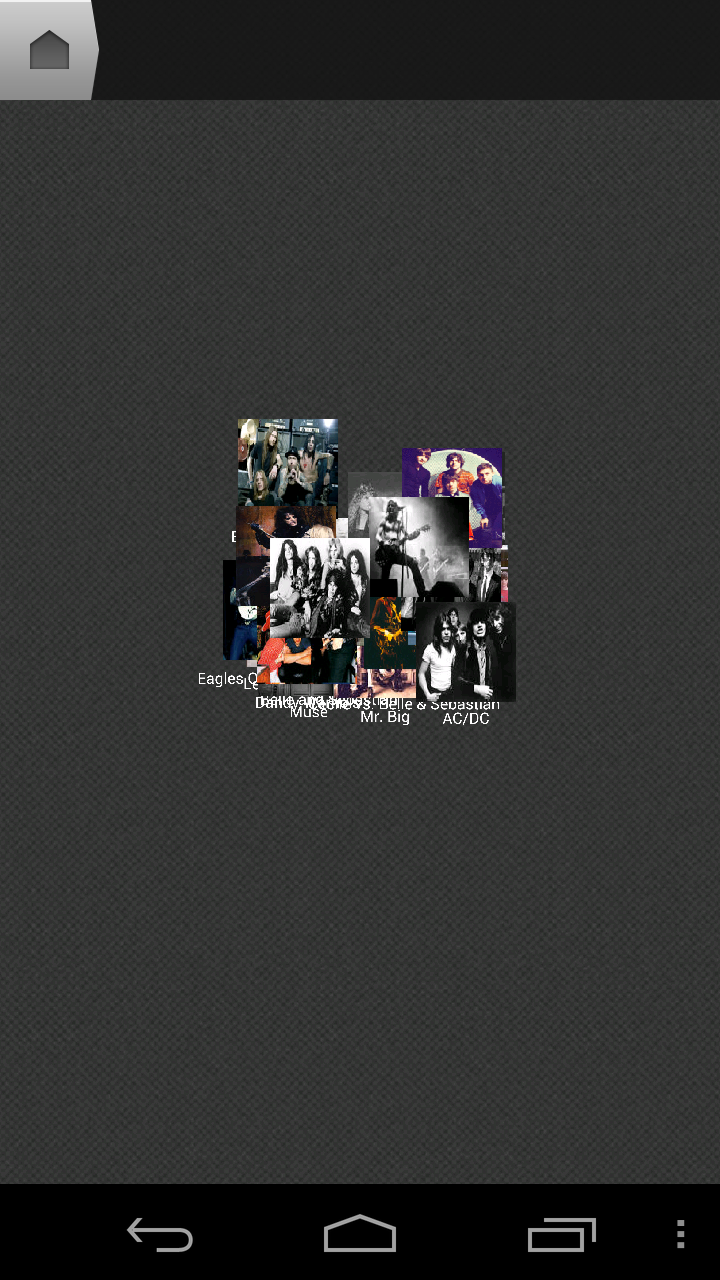
\includegraphics[width=0.4\textwidth]{figures/screen_mds_1_initial}
  \caption{The initial graph state before MDS calculation}
  \label{fig:screen_mds_1_initial}
\end{figure}

\newpage
\subsection{After 5 Subset Iterations (MDS)}
\label{subsec:mds-after-five-subset-iterations}

As previously described in sections ~\ref{sec:mds-algorithm} and ~\ref{sec:algorithm-assembly}, the first steps in the App's MDS computation are:

\begin{enumerate}
	\item Generation of a subset of 4 nodes, and
	\item Application of a number of spring model iterations on only this subset of 4 nodes.
\end{enumerate}

The screenshot depicted in figure ~\ref{fig:screen_mds_2_after_5_subset_iterations} shows the graph's state after five iterations of step 2. If compared to figure ~\ref{fig:screen_mds_1_initial}, it can be observed that four of the artist nodes (Airbourne, Chikinki, Keane, and Les Chameleons; their movements marked by arrows) have been moved to more outward positions.

\begin{figure}[H]
  \centering
    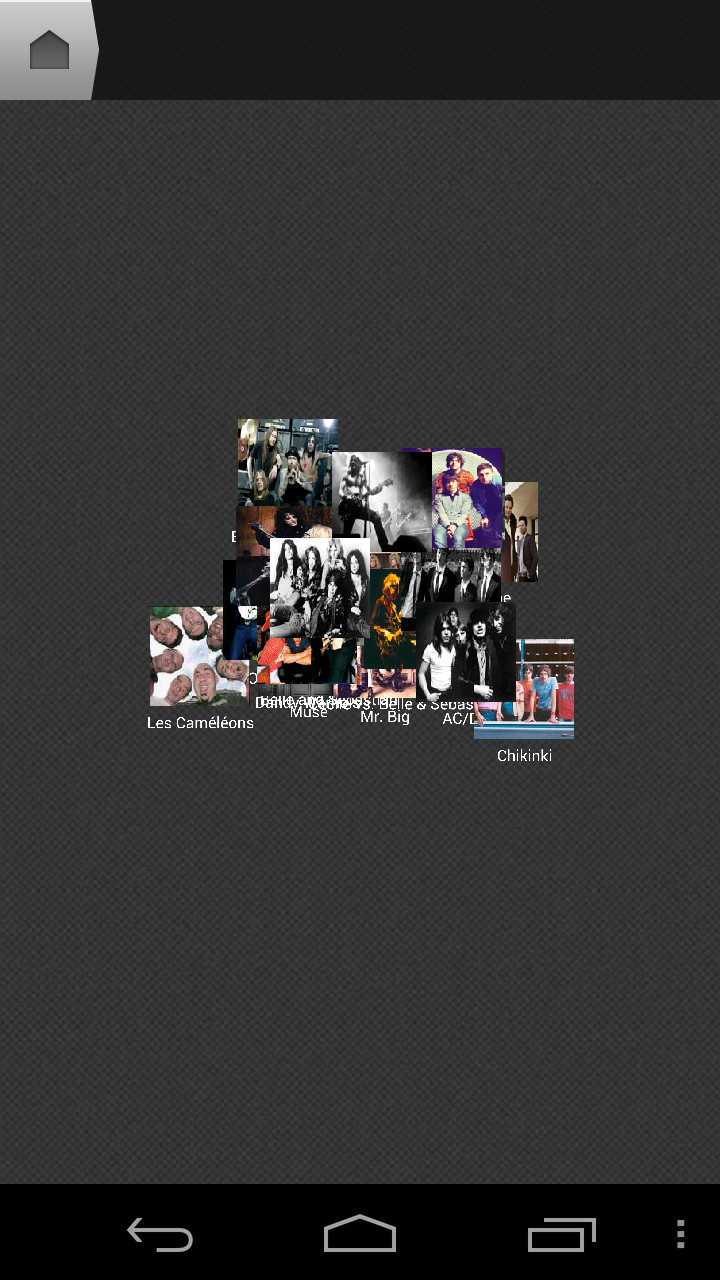
\includegraphics[width=0.4\textwidth]{figures/screen_mds_2_after_5_subset_iterations}
  \caption{Graph state after 5 iterations of the initial subset}
  \label{fig:screen_mds_2_after_5_subset_iterations}
\end{figure}

\newpage
\subsection{After 20 Subset Iterations (MDS)}

Similar to the previous figure, the following screenshot ~\ref{fig:screen_mds_3_after_20_subset_iterations} shows graph state during the second step (application of a number of spring model iterations on the initial subset) of MDS computation, but with 20 iterations of progress. It's easy to see that the four artist nodes (Airbourne, Chikinki, Keane, and Les Chameleons; which have already been moved in figure ~\ref{fig:screen_mds_2_after_5_subset_iterations}) have been displaced even more. The system stress for this subset of 4 nodes by now has fallen to almost zero (almost reached equilibrium), and further iterations will not move the nodes by much any more.

\begin{figure}[H]
  \centering
    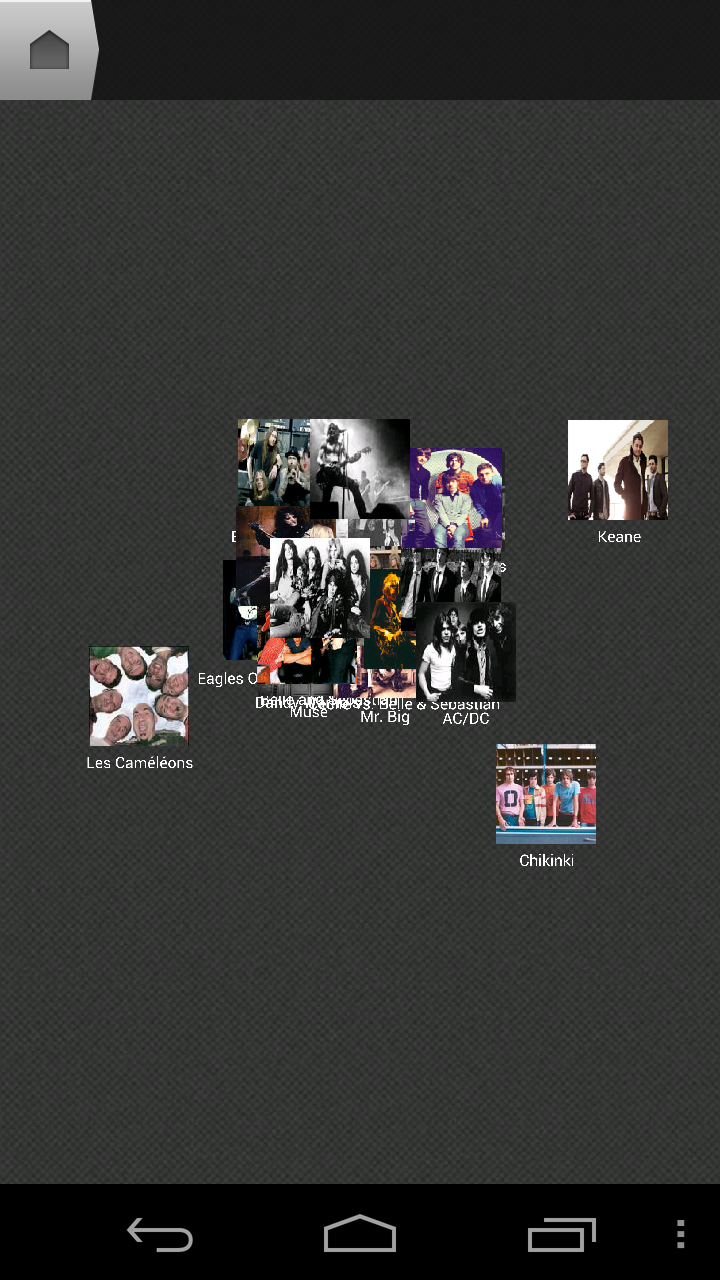
\includegraphics[width=0.4\textwidth]{figures/screen_mds_3_after_20_subset_iterations}
  \caption{Graph state after 20 spring force iterations of the initial subset}
  \label{fig:screen_mds_3_after_20_subset_iterations}
\end{figure}

\newpage
\subsection{After Placements of 5 Remaining Nodes (MDS)}

After spring model forces have been applied to the initial node subset, the remaining nodes (not being in the initial subset) are now placed in semantically sane positions. In figure ~\ref{fig:screen_mds_4_after_5_restnode_additions}, it can be observed that five nodes (AC/DC, Aerosmith, Alice Cooper, Arctic Monkeys, Oasis) have been moved to positions which differ from the old positions in the last screenshot (The new positions have been calculated by the algorithm described in section ~\ref{subsec:libraryvis}). 

\begin{figure}[H]
  \centering
    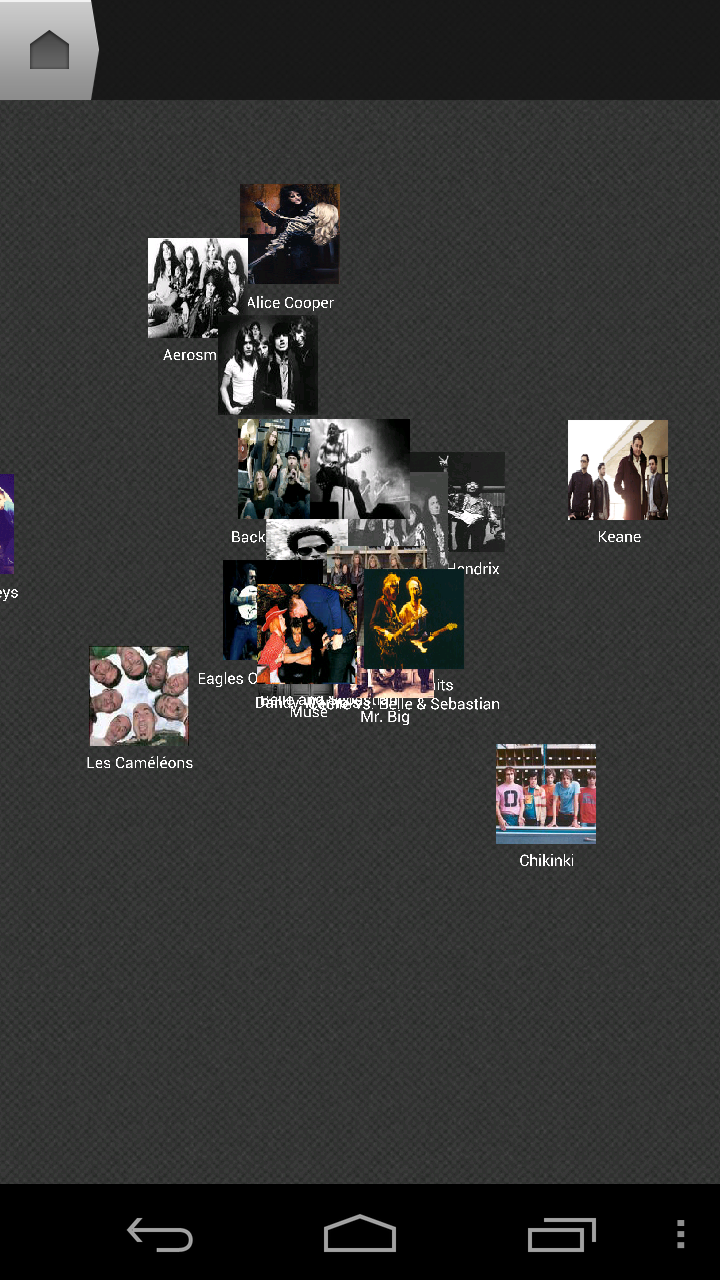
\includegraphics[width=0.4\textwidth]{figures/screen_mds_4_after_5_restnode_additions}
  \caption{Graph state after 5 placements of nodes outside the initial subset}
  \label{fig:screen_mds_4_after_5_restnode_additions}
\end{figure}

\newpage
\subsection{After Placements of All Remaining Nodes (MDS)}

Figure ~\ref{fig:screen_mds_5_after_all_restnode_additions} shows the graph's state after all nodes not in the initial subset have been placed in approximated positions. Although all nodes have been displaced at least once, this is an intermediate state, not yet resembling the algorithm's final outcome. Most nodes should be at least near their optimal position, minimizing system stress, but tests have shown that some nodes will be displaced by much in the following placement corrections. The reason for this is that the "'remaining nodes"' have been placed next to their most similar node (artist), but this position does in some cases not satisfy the spring model forces, and they have to move in order to correct the placement error. The amendment of these placement errors is the reason why the next step will perform a placement correction by re-applying the spring model algorithm on all artist nodes.

\begin{figure}[H]
  \centering
    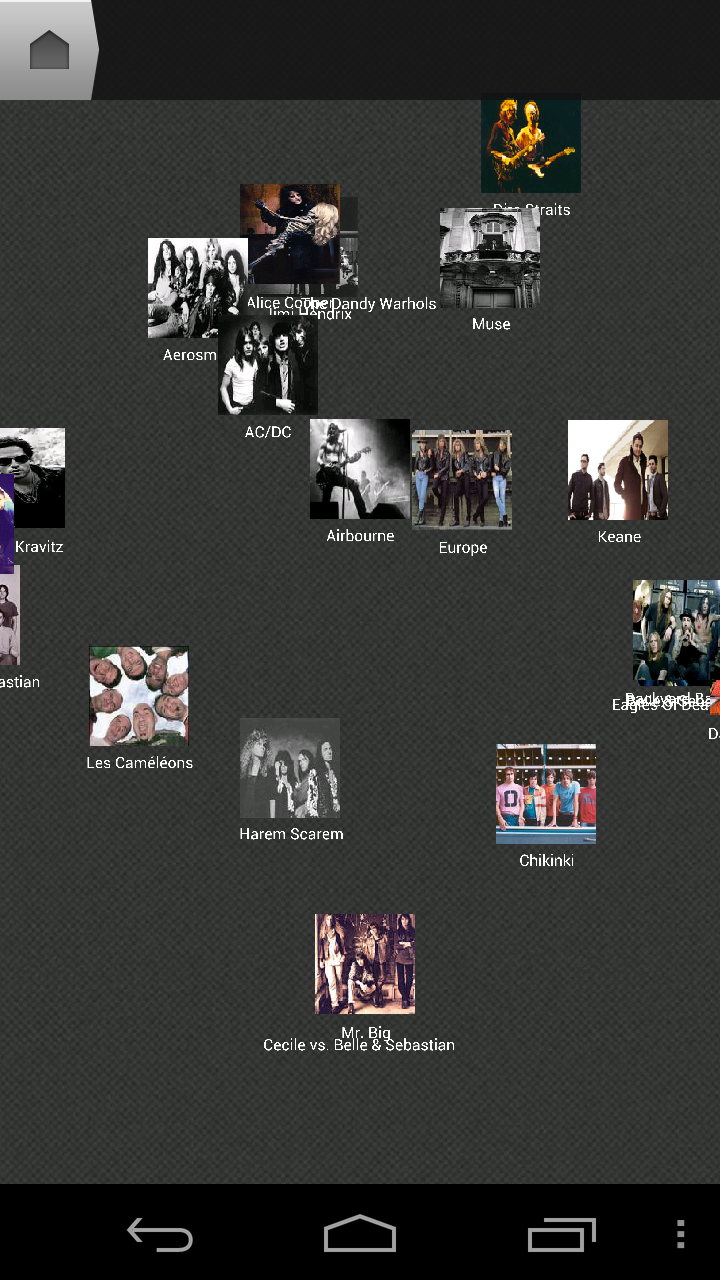
\includegraphics[width=0.4\textwidth]{figures/screen_mds_5_after_all_restnode_additions}
  \caption{Graph state after placements of all nodes outside the initial subset}
  \label{fig:screen_mds_5_after_all_restnode_additions}
\end{figure}

\newpage
\subsection{After 5 Placement Correction Iterations (MDS)}

Similar to the beginning of the calculations (depicted in Section ~\ref{subsec:mds-after-five-subset-iterations}), the spring model algorithm is again applied to the graph, but on all nodes at once. The previously approximated positions for many of the nodes have to be corrected (i.e., system stress has to be reduced) for the produced layout to increase significance. Application of a limited number of spring model iterations has the potential to improve the expressiveness of the layout greatly and reduce system stress. Figure ~\ref{fig:screen_mds_6_after_5_cleanup_iterations} displays graph state after five spring model iterations, reducing system stress by ~20 percent. Artist "'Mr. Big"' has been placed on a sub-optimal position by the previous algorithm steps, and after five correction iterations has now been moved upwards, as compared to the last screenshot.

\begin{figure}[H]
  \centering
    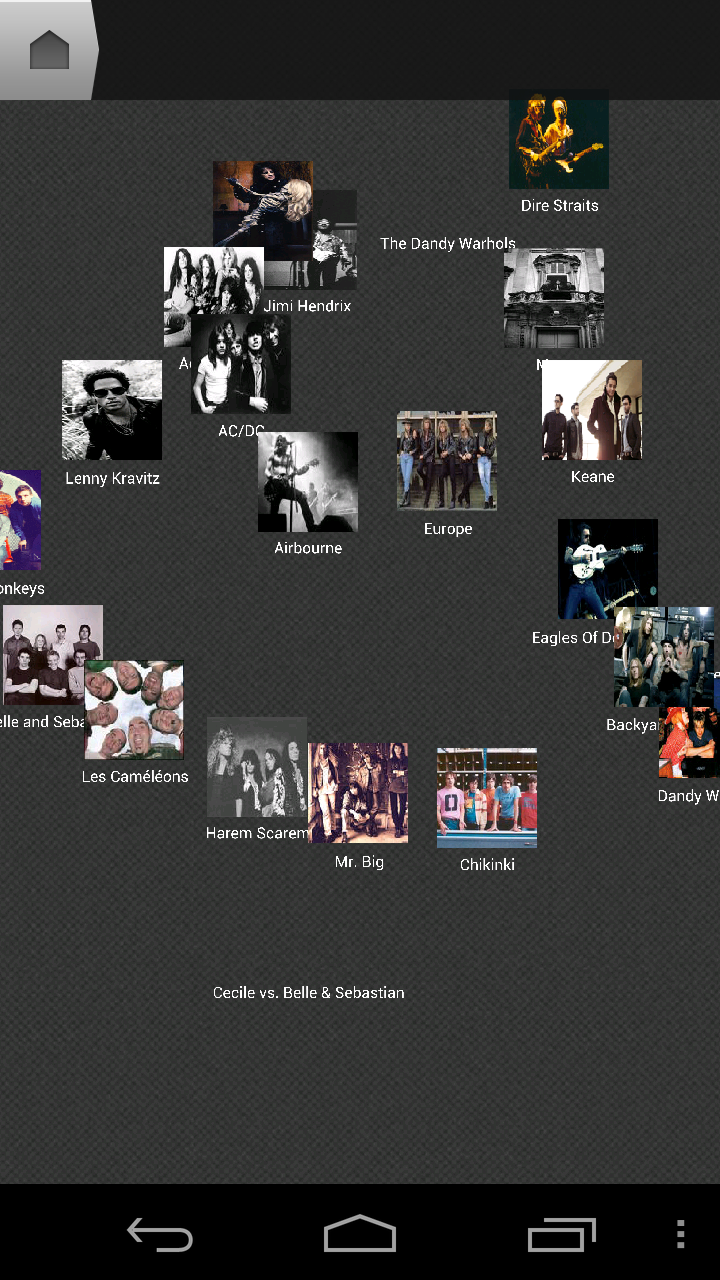
\includegraphics[width=0.4\textwidth]{figures/screen_mds_6_after_5_cleanup_iterations}
  \caption{Graph state after 5 spring model iterations of all nodes}
  \label{fig:screen_mds_6_after_5_cleanup_iterations}
\end{figure}

\newpage
\subsection{After 10 Placement Correction Iterations (MDS)}
\label{subsec:mds-after-ten-placement-iterations}

After 10 spring model iterations, the resulting layout features lower system stress than after 5 iterations (see last step). It can be observed in figure ~\ref{fig:screen_mds_7_after_10_cleanup_iterations} that nodes have not moved so much in this step as they moved in the previous step (going from 0 to 5 placement correction iterations).
The graph's nodes have been laid out such that their centers' positions reduce system stress - not giving any heed to overlappings. Therefore, the process does not end here, but these overlappings are eliminated in the next steps in order to prevent that any one node hides the other.

\begin{figure}[H]
  \centering
    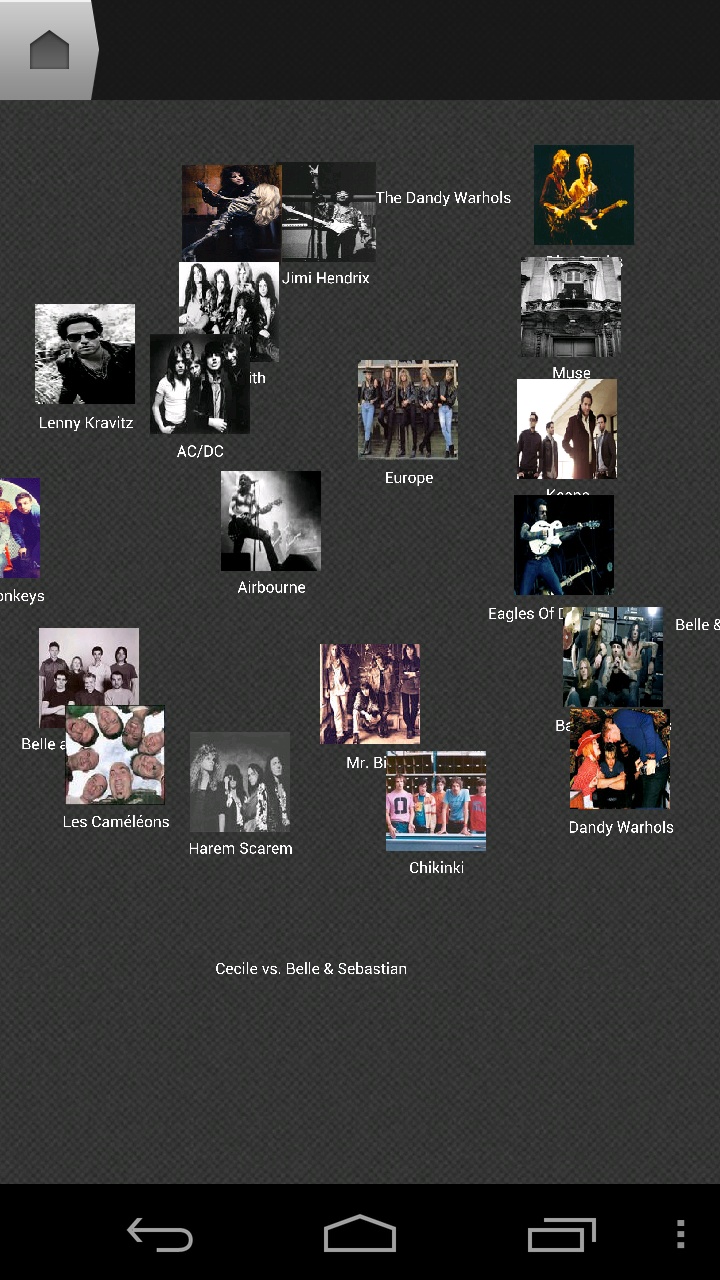
\includegraphics[width=0.4\textwidth]{figures/screen_mds_7_after_10_cleanup_iterations}
  \caption{Graph state after 10 spring force iterations of all nodes}
  \label{fig:screen_mds_7_after_10_cleanup_iterations}
\end{figure}

\newpage
\subsection{After Removal of Node Overlappings from 5 Nodes}

By applying the algorithm for removal of node overlappings described in section ~\ref{sec:removal-node-overlapping}, overlapping artist nodes are separated from each other. Figure ~\ref{fig:screen_mds_8_after_5_uncollided_nodes} shows the graph's state after five nodes have been processed. Two artists have not been moved because they did not overlap with other artists, but three artists (Aerosmith, Airbourne, Alice Cooper) have been moved, i.e. they have been repositioned such that they keep a certain margin to any other nodes.

\begin{figure}[H]
  \centering
    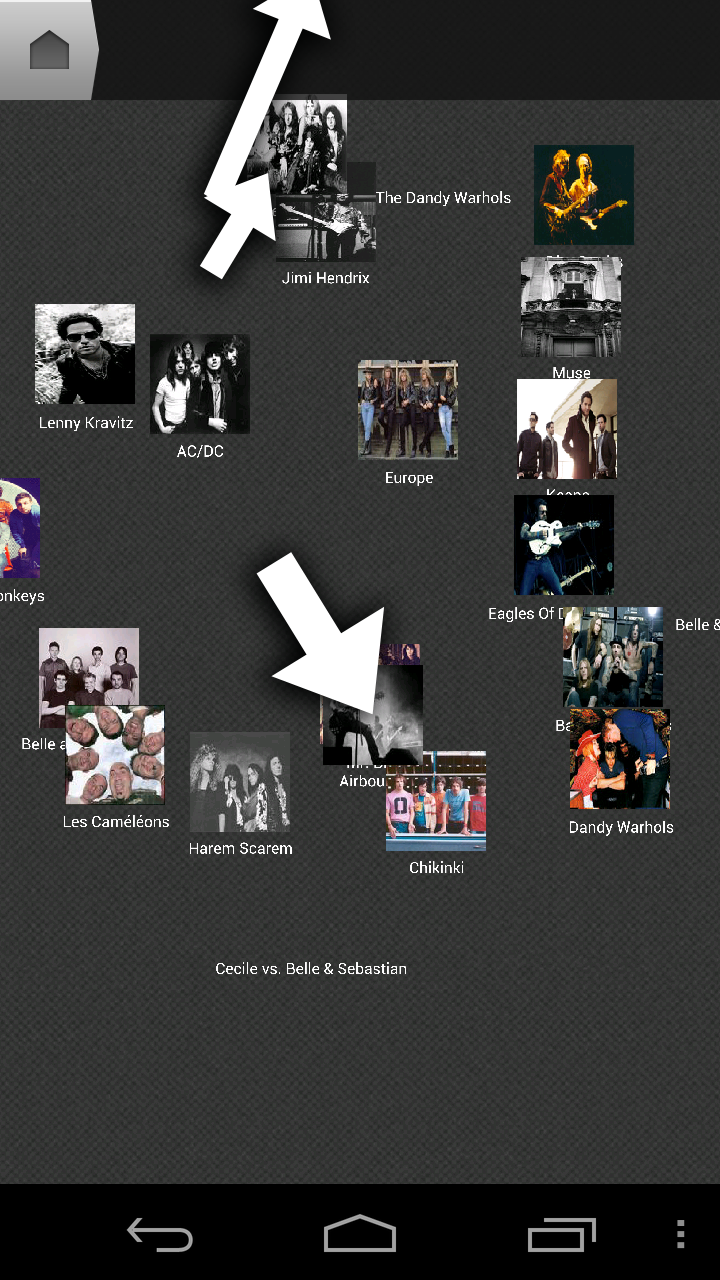
\includegraphics[width=0.4\textwidth]{figures/screen_mds_8_after_5_uncollided_nodes}
  \caption{Graph state after removal of node overlappings from 5 nodes}
  \label{fig:screen_mds_8_after_5_uncollided_nodes}
\end{figure}

\newpage
\subsection{After Removal of Node Overlappings from Half of All Nodes}

As a continuation of the last screenshot, the following figure ~\ref{fig:screen_mds_9_after_half_uncollided_nodes} depicts the graph's state after half of all artist nodes have been repositioned to avoid overlappings.

\begin{figure}[H]
  \centering
    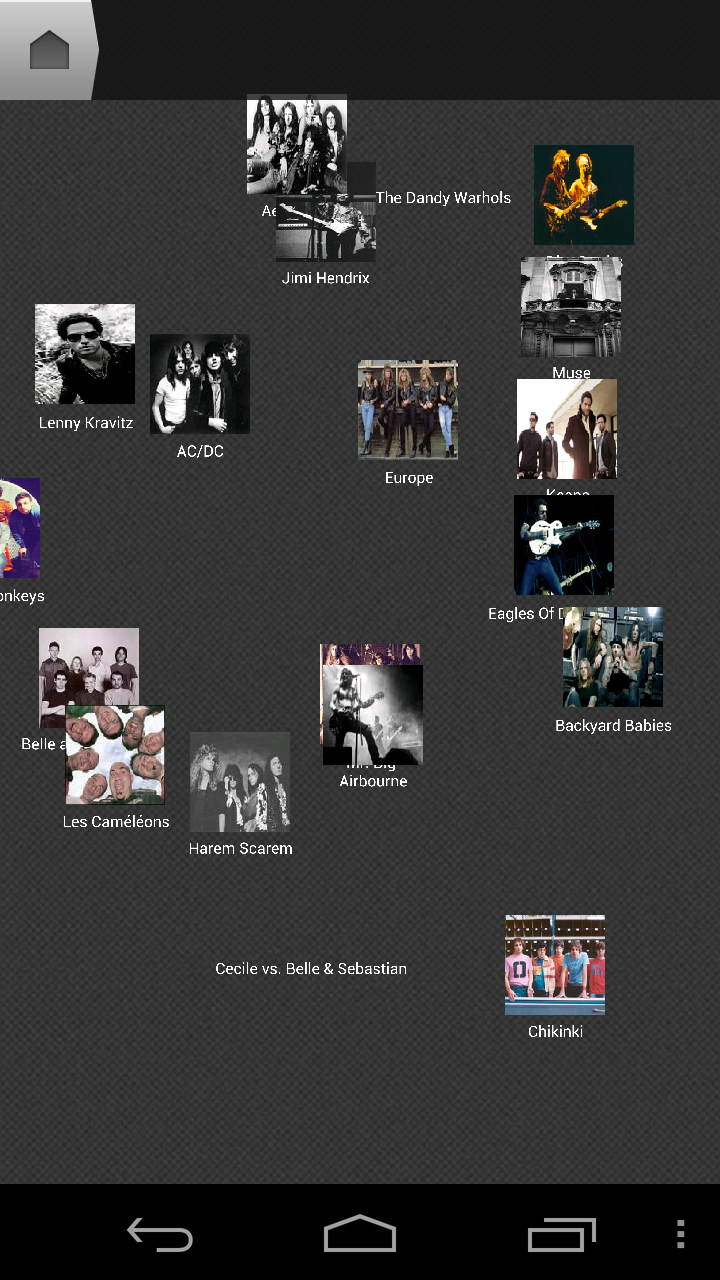
\includegraphics[width=0.4\textwidth]{figures/screen_mds_9_after_half_uncollided_nodes}
  \caption{Graph state after removal of node overlappings from half of all nodes}
  \label{fig:screen_mds_9_after_half_uncollided_nodes}
\end{figure}

\newpage
\subsection{After Removal of Node Overlappings from All Nodes}

Screenshot ~\ref{fig:screen_mds_10_after_all_uncollided_nodes} shows the final state of the graph, at the end of all computations. This is a compromise between the intermediate result shown in subSection ~\ref{subsec:mds-after-ten-placement-iterations}, and a user-friendly (easy to grasp) representation of the graph. Clearly, system stress has been increased by removal of node overlappings; but, the process has made the MDS algorithm's results readable and easily understandable. The resulting margin between the nodes is subject to adjustable parameters, leaving room for further optimization.

In the actual App implementation, this is the first state displayed to the user - all previous states are hidden from her. Subsequently, the App reacts to touch gestures in order to enable navigation and exploration of the structure on small screens (it's understood that screenshot~\ref{fig:screen_mds_10_after_all_uncollided_nodes} does not show all artists of the graph).

\begin{figure}[H]
  \centering
    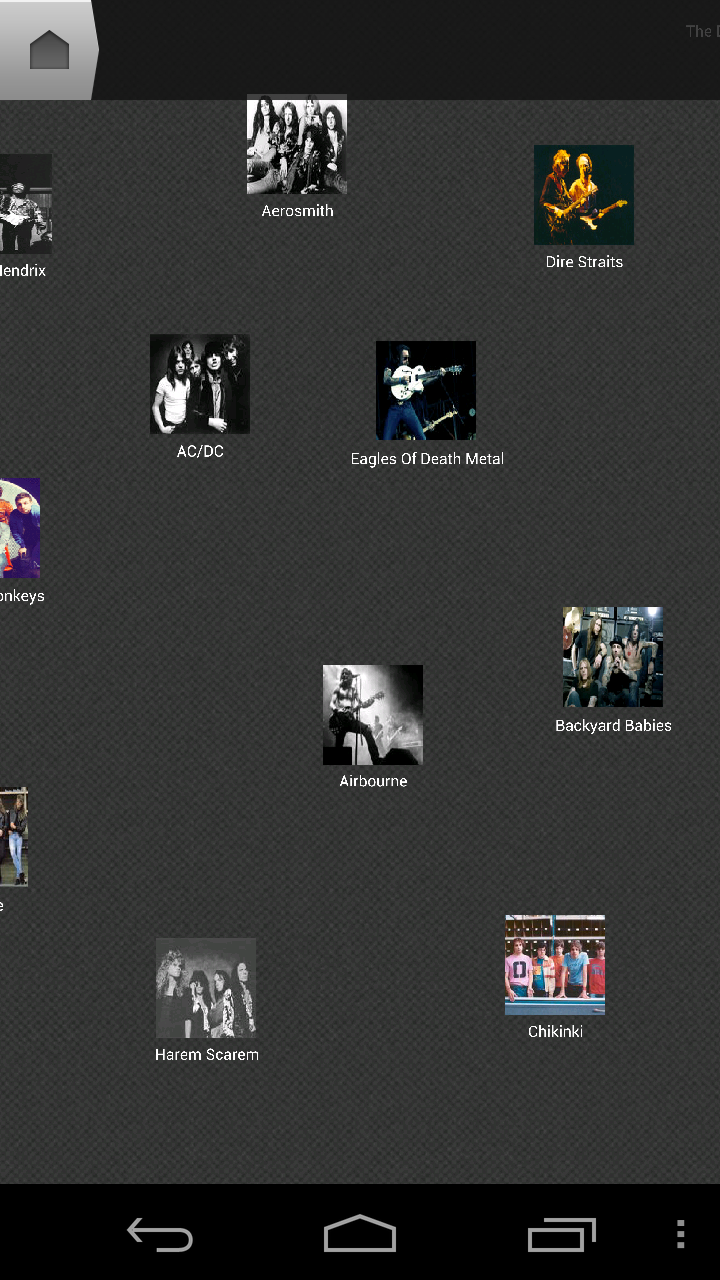
\includegraphics[width=0.4\textwidth]{figures/screen_mds_10_after_all_uncollided_nodes}
  \caption{Graph state after removal of node overlappings from all nodes}
  \label{fig:screen_mds_10_after_all_uncollided_nodes}
\end{figure}

\section{Retrieval of Music Metadata}

\subsection{Querying of Music Metadata on the Device}

Android has a cursor-based query system for multimedia metadata (kept up-to-date transparently by the operating system). Creation of a cursor for all artists on the device is performed by program code like this:

\begin{verbatim}
Cursor artistCursor = mContext.getContentResolver().query(
	MediaStore.Audio.Artists.EXTERNAL_CONTENT_URI,
    artistProjection, null, null, null);
\end{verbatim}

Since the returned metadata also contains a unique key for each multimedia file, metadata can be
persisted in a database and later be reused without obstacles.
Metadata records themselves contain as much data as the user or the file-generating utility has defined
before the file was copied onto the device - clearly, files may not have any metadata available at all.

In the implementation of the App, such a cursor is traversed over all available music titles, and several entities are derived:

\begin{itemize}
	\item Artist,
	\item Album, and
	\item Track title.
\end{itemize}

While these entities are created, the implementation checks whether they already exist, and skips creation accordingly. Retrieved data is then stored in the App's on-device database.

\subsection{Retrieval of Music Metadata from Web Sources}

Last.fm \cite{url:lastfm} and Echonest \cite{url:echonest} are the de facto standards for music metadata retrieval in the world wide web, 
at the time of writing of this paper. The author has chosen to use both of these services for retrieval 
of semantic metadata for the implementation. 

After the device's music titles and their metadata have been retrieved, their metadata has to be augmented or corrected with the normalized data from external sources - Last.fm and Echonest. To ensure a stable mapping from on-device to remote music metadata records, these are fetched up front. For every artist, album, and track the App has retrieved from the device, a match is searched for in web sources. Search for matches is performed by sending an ordinary search query to the web sources, and metadata records are returned as a result. Excerpts of the acquired records are then stored in the App's on-device database, as described in section ~\ref{sec:matching-music-entities}.

\section{Retrieval of Similarity Data}

Ideally, the retrieval of similarities between artists should provide an exhaustive list of similarities between any two artists. But, as a real-world implementation must make do with actuality, workarounds had to be found which provide approximations to artist similarities.
Echonest's artist similarity results contain no similarity metric, but only the implicit ranking of artists. Therefore, the author of this thesis decided \textbf{not to use Echonest's similarity metrics}.

Last.fm's artist similarity data is, in contrast to Echonest, augmented with accurate similarity measures in the range of $[0 .. 1]$. But, it is not possible to query Last.fm for a certain similarity relationship between two certain artists - instead, the top 100 similar artists for a certain artist can be retrieved together with the corresponding similarity values. It's clear that this way, many artist-to-artist relations in a music collection will not receive a similarity measure. Instead, a dedicated algorithm has to approximate similarity values which were not provided by Last.fm. This algorithm is shown in listing ~\ref{alg:similarity-approximation} in  appendix ~\ref{app:algorithm}.


\section{Visualization Details}

Apart from the previously described computational algorithms, the App features a number of components or behavior not contained in the Android operating system. In the following, the most interesting features aiding the visualization of content will be described.

\subsection{Drawing with OpenGL}

Android provides App developers with the possibility to implement three-dimensional viewports in OpenGL ES \cite{url:opengles}, which is a downsized version of ordinary OpenGL and meant for implementation in handheld devices. OpenGL is a specification which is used as a blueprint by operating systems vendors and GPU producers alike. An OpenGL context can be seen as a state-machine which is manipulated by external API calls.

While the prototype shall implement a 2D visualization, its implementation in OpenGL (which is a 3D drawing specification) is necessary to provide a reasonably high framerate. Early prototype tests with a strict 2D implementation (Android 2D canvas drawing) showed that image rendering let the framerate drop considerably, so that viewport zooming, panning, and animations were no longer smooth to the human eye. The app's usability suffered from this, and so the prototype was rebuilt using OpenGL. The reason why OpenGL performs better in this context is that GPUs are better suited for handling images (textures) than CPUs, because their architecture and instruction sets are primarily dedicated to rendering.

In order to be able to employ OpenGL for graph rendering, the author of this thesis had to create a number of abstract meta classes and find a way to resemble user interactions in the drawn 3D picture. As mentioned before, the objective was to draw pseudo-2D, such that all music objects are displayed as pictures, viewed from the top. Accordingly, the viewport has to move sideways when the user moves one finger over the touchscreen, and it has to change its distance to the graph objects when the user zooms.

\subsection{Touchscreen Handling}

With the advent of smartphones, strong conventions have been established by phone vendors which determine how users may interact with the smartphone. Touchscreen technology provides a more immediate way of interaction than previous systems, allowing users to seemingly interact with the very objects they want to manipulate (as opposed to moving views and cursors with hardware buttons).
There are three touchscreen gestures supported by the App's implementation:

\begin{itemize}
	\item \textbf{Panning/Scrolling} - The user taps the finger onto the screen surface, does not let 
	go, and pulls the finger across the surface.
	\item \textbf{Zooming} - The user rests two fingers on the screen surface, and changes the distance	between her finger tips. If the distance decreases, then the zoom factor will increase; and vice versa.	Ideally, the reference points (which are touched by the user's fingers when she placed her fingertips on the screen) would always overlap with the user's fingertips, meaning that while the fingertips contract or pull apart, the zoom level would adapt such that the reference points stay beneath the fingertips. However, in the built App prototype, this has been considered out of scope, because of the three-dimensional nature of the OpenGL	rendering process making it difficult to achieve this effect.
	\item \textbf{Tapping} - The user taps her finger onto the screen surface at a point on which the
	desired object is located, and lets go again immediately. The App then reacts to this interaction
	with an adequate response or action, depending on the current state of the user interface.
\end{itemize}

\subsection{Animations}

To make transitions between view states in the App smoother and easier to follow for users, animations have been implemented to do so. It has been shown in an empirical study that comprehension of changes can be improved by adding animations ~\cite{Schlienger:2007}.

\textbf{Whole-screen transition} - If the user chooses to display an artist's albums, the transition to the next Activity (fullscreen Android layout component) is implemented as a fade-over animation, meaning that the second screen is added as an overlay and its alpha channel is animated from 0 to 1. This way, the user is able to notice the change of context without being disturbed by untraceable changes.

\textbf{Artist Node animation} - If the user selects an artist by tapping, the artist's image depiction is moved on the z-axis towards the virtual camera - appearing nearer to the viewport. This puts an emphasis on the selected artist and makes for a pleasing optical effect. As OpenGL is a low-level framework, animations like this have to be implemented by the developer - keeping track of animation start and projected end time, and determining the state for every newly drawn frame.

\textbf{Context-related graph area darkening} - If the user chooses to display a seed artist's related (similar) artists, the graph area darkens over all other currently displayed artists, to put an emphasis on the selected artist and its related artists. This effect is achieved by overlapping all other previously shown contents with a semitransparent, by placing it between the emphasized artists and the other artists z-wise. Its opacity value is at first set to zero and then animated to 60 percent, achieving an effect of continuous darkening of all artists except the seed artist and its related artists over a short period of time (200 milliseconds).

\section{Structure of the App}

The prototypical App implementation is targeted at the Android operating system. In this section, some implementation specifics will be given for better reproducability.

\subsection{Activities}

The App's UI stack consists of two Activities (screens):

\begin{itemize}
	\item \textbf{Loading Activity} - Fetching metadata from the internal storage and web sources, and compilation of the same is a lengthy process, and therefore a dedicated Activity exists in the App, displaying progress indicators.
	\item \textbf{Artists Activity} - The main screen of the App, showing all artists in the user's music collection, laid out such that nearness between artists implicates similarity.
	\item \textbf{Albums Activity} - The secondary screen, displaying an artist the user has selected on the previous screen, along with their albums.
\end{itemize}

The apps' package and class structure is listed in appendix ~\ref{app:packages}.

\subsection{Third Party Libraries}

\begin{itemize}
	
	\item \textbf{jEn-api}, an Echonest API library for Java, also working in Android apps. \\
License: \emph{New BSD License}

	\item \textbf{lastfm-java}, an unofficial Last.fm API library for Java, also working in Android apps. \\
License: \emph{New BSD License}

	\item \textbf{ORMLite}, a low-profile object relational mapper for SQLite in Java, also working in Android apps. \\
License: \emph{ISC License}

	\item \textbf{JSON.simple}, a JSON (JavaScript Object Notation) parser for Java, also working in Android apps. \\
License: \emph{Apache 2.0 License}

	\item \textbf{Android Support Library v4}, a library provided by Google to enable more recent Android features for older OS versions. \\
License: \emph{Apache 2.0 License}

	\item \textbf{Android Annotations}, a compile-time library which generates code from Java annotations, to allow pseudo-dependency injection and more advanced features. \\
License: \emph{Apache 2.0 License}

\end{itemize}

\section{Summary}

This chapter has explained the components, algorithms, and concepts used to construct a prototype demonstrating the visualization of artist similarity, runnable on mobile Android devices.

Algorithms and the flow of information between them has been described, both for the visualization of a music library (on-device metadata extraction, matching, web source metadata extraction and interpolation, layout generation, removal of node overlappings, display of the graph to the user), and for artist discovery (querying of related artists from web sources, their integration into the layout, and continuous rearrangement via a force-based layout algorithm).
Thereafter, different states of the App prototype while executing the previously described algorithms have been illustrated, using screenshots.

Retrieval of music metadata from the user's device and web sources, and retrieval of similarity data from web sources has been described in detail. Since this similarity data may be incomplete, an interpolation algorithm for unknown values has been given.
A part of the MDS algorithm (already described in length in Chapter ~\ref{ch:computation}), the  positioning of graph nodes based on system stress minimization, has been detailed as pseudocode. The algorithm for the removal of node overlappings in the graph was also shown.
To provide some details about visualization and the App's user interaction model, OpenGL drawing, touchscreen gestures, and animations were elaborated on.

Finally, a short introduction to the Android operating system was given, and the prototype App's structure (Activities and other classes) and third party libraries were detailed.